\documentclass{article}
\PassOptionsToPackage{round,authoryear}{natbib}
\usepackage[sglblindworkshop]{neurips_2026}
\workshoptitle{E-Values: From Statistics to ML}

\usepackage[utf8]{inputenc}
\usepackage[T1]{fontenc}
\usepackage{hyperref}
\usepackage{url}
\usepackage{booktabs}
\usepackage{amsmath,amssymb}
\usepackage{amsfonts}
\usepackage{nicefrac}
\usepackage{microtype}
\usepackage{graphicx}

\newtheorem{lemma}{Lemma}

\title{An Exact Conditional Null for Correlated Failure in Open-Model \\
Ecosystems, and a Route to Anytime-Valid Monitoring}

\author{
  Shaurya Gupta \\
  Independent Researcher \\
  Mumbai, India \\
  \texttt{shauryaguptaa8@gmail.com}
}

\begin{document}

\maketitle

\begin{abstract}
Measuring correlated failure between language models requires a null hypothesis for
``independent enough,'' and prior work shows the conclusion is highly sensitive to which null is
chosen, leaving the choice apparently subjective. We show one null is not a choice: the row and
column margins of a model-by-item outcome matrix are the jointly sufficient statistics of the
Rasch family, so the uniform distribution over margin-matched matrices is the unique exact,
fit-free conditional null for that family. At this null, on $1{,}228$--$1{,}362$ open models
across five benchmarks, the commonly reported mean-level ``excess'' co-failure is a deterministic
function of item difficulty and vanishes identically, while a genuine second-order residual
correlation of $2.8$--$11.8\times$ its null survives, is robust to removing near-duplicate models,
and concentrates in a handful of latent dimensions. Our test is currently a fixed-sample exact
randomization test. We argue the same conditional null is the natural fixed-sample building block
for an anytime-valid monitor of correlated failure as an open-model ecosystem grows, and sketch
the construction as an open problem for this workshop.
\end{abstract}

\section{Motivation}

If many deployed models share blind spots, an ensemble, a panel of model judges, or a market of
competing screening vendors supplies far less independent evidence than its headcount suggests.
Measuring this requires comparing the rate at which models fail the same items against a baseline
in which failures are independent. \citet{jo2026} show this comparison is highly sensitive to the
assumed baseline: conditioning on item difficulty attenuates residual correlations, ``some even
flipping from strongly positive to slightly negative,'' and they prove that a sufficiently
expressive null can explain away any observed dependence. Their stated conclusion is that the
choice of null is subjective. This paper argues the ladder of nulls has a canonical rung, reports
what the exact answer is there, and points at what this workshop's machinery could add to it.

\section{The canonical null}

Let $F \in \{0,1\}^{N\times M}$ record $F_{im}=1$ iff model $i$ fails item $m$, with row sums
$r_i$ and column sums $c_m$. The Rasch model $\Pr(F_{im}=1)=\sigma(\alpha_i+\beta_m)$ has
$\{r_i\}$ and $\{c_m\}$ as jointly sufficient statistics. Conditioning on both therefore
eliminates $\alpha$ and $\beta$ exactly: the conditional law of $F$ given its margins is uniform
on the set of margin-matched binary matrices, for every parameter value \citep{rasch1960}. That
set is the ecologists' fixed-fixed null, and we sample it with curveball \citep{strona2014}, whose
convergence to uniform on the fibre is proved by \citet{carstens2015} and which we verify directly
by enumeration on four small fibres. Unlike a fitted item-response null, this null requires no
optimizer, no penalty, and no identification convention — it is the strongest ability-and-difficulty
control obtainable without fitting anything, and it is unique in that respect.

\begin{lemma}[Mean co-failure depends only on item margins]
$O = \frac{1}{MN(N-1)}\sum_m (c_m^2 - c_m)$.
\end{lemma}
\noindent Consequently any randomization preserving the item margins leaves the mean pairwise
co-failure rate $O$ invariant with exactly zero variance: the reported ``excess'' co-failure at
this null is identically zero by construction, not empirically small. This degeneracy is
independently known in ecology (Schluter's V-ratio), psychometrics (Cronbach's $\alpha$), and
inter-rater agreement (Fleiss), none of which is cited in the model-evaluation literature that
reports it; we state the identities and attribute them in the full paper.

\section{What survives at the exact null}

Table~\ref{tab:neff} reports the participation ratio of the conditioned residual-correlation
spectrum against its exact-margin null, on the archived Open LLM Leaderboard
($1{,}228$--$1{,}362$ models, five benchmarks, harvested at zero inference cost by reading only
the metric column of each result file). The observed value sits at $2.8$--$21.4\%$ of the null.
Uncalibrated, the same statistic reads $1.5$--$3.6$ on every benchmark — a number driven almost
entirely by the single shared item-difficulty eigenvalue the conditioning removes, and easily
misread as ``near-total redundancy'' before calibration. We show algebraically that this
statistic cannot separate one weak global factor from a partition into tight clusters, and we use
spectral diagnostics instead: on ARC, the leading eigenvalue explains only $54\%$ of squared
residual mass (a single shared factor would give $\approx 99\%$), and six eigenvalues exceed the
null's spectral edge. The result is robust to removing near-duplicate models (on ARC, discarding
$900$ of $1{,}362$ near-clones moves the ratio from $23.6$ only to $29.0$) and to a
$2.8\times$-larger replication population collected six weeks later, where every ratio moves by
at most $0.010$.

\begin{table}[t]
\centering
\small
\begin{tabular}{lrrrrr}
\toprule
Benchmark & $N$ & $N_{\text{eff}}$ obs. & $N_{\text{eff}}$ null & ratio & rms excess ($\times$ null) \\
\midrule
ARC-Challenge & 1362 & 23.6 & $449.3\pm3.4$ & 0.052 & $5.5\times$ \\
Winogrande & 1361 & 20.1 & $493.8\pm3.0$ & 0.041 & $4.6\times$ \\
TruthfulQA & 1334 & 17.4 & $309.7\pm2.4$ & 0.056 & $4.1\times$ \\
GSM8K & 1228 & 118.6 & $553.1\pm2.2$ & 0.214 & $2.8\times$ \\
HellaSwag & 1362 & 27.3 & $958.0\pm3.2$ & 0.028 & $11.8\times$ \\
\bottomrule
\end{tabular}
\caption{Effective independent models after exact-margin conditioning, all five benchmarks. The
null column is the mean and SD of $400$ curveball replicates with both margins exactly preserved.}
\label{tab:neff}
\end{table}

\begin{figure}[t]
\centering
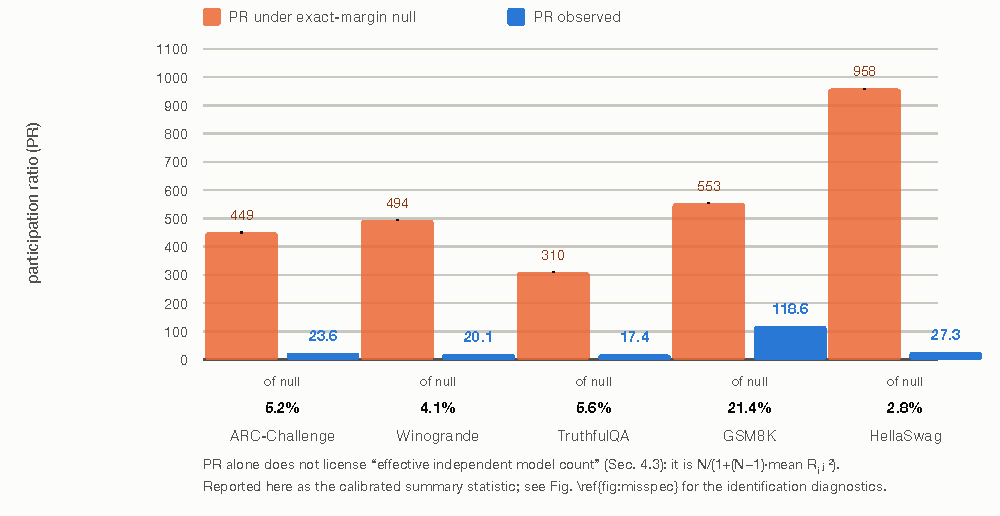
\includegraphics[width=0.85\linewidth]{../../../figures/fig_residual_summary.pdf}
\caption{Observed participation ratio against its exact-margin null, all five benchmarks. Reported
here as a calibrated summary statistic, not as a literal count of independent models
(Section~\ref{sec:evalues}'s test cannot distinguish one weak factor from tight clusters).}
\label{fig:residualsummary}
\end{figure}

A pre-registered dispersion statistic (the variance of pairwise co-failure) was our primary
planned test and it failed its own kill condition, coming out inconsistent in sign across
benchmarks; we report it as refuted rather than reinterpreted. What survives is the second-order
spectral structure above, not the first statistic we planned to report — a distinction we think
matters for how confirmatory claims about model diversity should be validated in this literature.

\section{Toward an anytime-valid version}
\label{sec:evalues}

Everything above is a fixed-$n$ exact test: for a fixed population of $N$ models, curveball gives
Monte Carlo draws from the exact conditional distribution, and the observed statistic is compared
against them once. The population it is computed on is not actually fixed — the Open LLM
Leaderboard and its successors add new open models continuously, and a natural downstream use of
this test is a standing monitor: ``has correlated failure in the open ecosystem gotten worse since
last quarter,'' checked repeatedly as new submissions arrive, without the type-I error inflation
that repeated testing on a growing sample otherwise incurs. That is exactly the anytime-valid
inference problem this workshop's community formalizes with e-values and test martingales
\citep{shafer2021,vovkwang2021,ramdas2023,grunwald2024}.

We see two routes and neither is worked out here. First, one could construct a test martingale
directly from the exact conditional law: since the conditional distribution of $F$ given its
margins is uniform on a fully specified finite set for every model added, each new model's
observed row is itself a draw whose conditional distribution under the null is known exactly (not
merely asymptotically), which is the situation in which e-value construction from a likelihood
ratio against a composite alternative is most tractable. Second, since our headline statistic is
already a Monte Carlo $p$-value against an exact reference distribution, one could wrap it in a
merging or calibration scheme that converts a sequence of such $p$-values into an e-process,
trading some power for the anytime-validity guarantee. The obstacle in both cases is that new
models are not exchangeable arrivals in the usual online-testing sense: they are added by
submitters who observe the current leaderboard, so any construction has to either condition away
that selection effect or treat it explicitly — a version of the same population-dependence
objection \citet{jo2026} raise about a fixed null, now posed sequentially. We flag this as the
concrete open problem we would bring to this workshop, not as a result: the exact conditional null
is, we think, the right fixed-sample primitive to build an anytime-valid ecosystem monitor on top
of, but we have not yet built one.

\section{Limitations}

Claims cover the evaluated open-model ecosystem on multiple-choice-style benchmarks, not deployed
proprietary systems. Our conditioning model is unidimensional (Rasch); a misspecification check
shows two-parameter discrimination heterogeneity alone cannot reproduce the observed effect size,
but a low-dimensional multi-ability structure can reproduce much of it, so we cannot fully
separate genuine behavioral concentration from an underfit null family. All code, data, and the
pre-registration (with dated amendments) are archived and linked in the full paper.

\begin{thebibliography}{9}
\small
\bibitem[Carstens(2015)]{carstens2015} C.~J. Carstens. Proof of uniform sampling of binary matrices with fixed row sums and column sums for the fast Curveball algorithm. \emph{Physical Review E}, 91:042812, 2015.
\bibitem[Gr{\"u}nwald et al.(2024)]{grunwald2024} P.~Gr{\"u}nwald, R.~de Heide, and W.~Koolen. Safe testing. \emph{Journal of the Royal Statistical Society Series B}, 86(5):1091--1128, 2024.
\bibitem[Jo et al.(2026)]{jo2026} N.~Jo, N.~Garg, and M.~Raghavan. The subjectivity of monoculture. \emph{arXiv:2602.24086}, 2026.
\bibitem[Ramdas et al.(2023)]{ramdas2023} A.~Ramdas, P.~Gr{\"u}nwald, V.~Vovk, and G.~Shafer. Game-theoretic statistics and safe anytime-valid inference. \emph{Statistical Science}, 38(4):576--601, 2023.
\bibitem[Rasch(1960)]{rasch1960} G.~Rasch. \emph{Probabilistic Models for Some Intelligence and Attainment Tests}. Danmarks P\ae dagogiske Institut, 1960.
\bibitem[Shafer(2021)]{shafer2021} G.~Shafer. Testing by betting: A strategy for statistical and scientific communication. \emph{Journal of the Royal Statistical Society Series A}, 184(2):407--431, 2021.
\bibitem[Strona et al.(2014)]{strona2014} G.~Strona, D.~Nappo, F.~Boccacci, S.~Fattorini, and J.~San-Miguel-Ayanz. A fast and unbiased procedure to randomize ecological binary matrices with fixed row and column totals. \emph{Nature Communications}, 5:4114, 2014.
\bibitem[Vovk \& Wang(2021)]{vovkwang2021} V.~Vovk and R.~Wang. E-values: Calibration, combination, and applications. \emph{Annals of Statistics}, 49(3):1736--1754, 2021.
\end{thebibliography}

\end{document}
